Our experiments using our inter-cloud systems yield promising support for this approach.  Our experiments show only a slight degradation of information availability as a result of our network permeated security approach, with redaction and rerouting demonstrating the smallest degradation at a higher impact on delivered information integrity.  Encryption-based approaches have the most performance degradation, but have a smaller impact on information integrity.

In these tests, we used a simulated $\gamma$-categorized system.  This is the kind of system that organizations like the UCDMO have identified as the final goal state of their work, systems that incorporate policy-centric management in the fabric of systems and networks (12).  The kind of components required to do this kind of policy-based content-sensitive evaluation do not currently exist, and components of these kinds of systems are only now beginning to emerge.  Systems like OpenFlow, when they have stronger hardware support, can begin to provide some of these kinds of capabilities.  OpenFlow enabled systems are not yet common or widely used however, and though they do provide the needed control for these kinds of systems, the do not supply the necessary policy interpretation and evaluation.  As a result, this experimental work was conducted over an HTTP overlay network, at the application layer.  Using a document-focused protocol makes content evaluation simpler as well, as systems can evaluate all content when it transits a network rather than maintaining a buffer of content required when processing packet-level communications.

In order to develop a stronger perspective on the network performance, we measure delivery times from three separate nodes.   One node is hosted in Comcast's infrastructure (a large local Internet Service Provider), one at Amazon, and another at Rackspace.  The tested network has four levels.  The first level has a single router node.  The next level has two routers, both connected to the router in the first level.  The third level contains four routers, two attached to each of the routers at the level just above.  Finally, the fourth level contains nodes, distributed so that two level three routers have three nodes, one level three router has two nodes, and the last level three router has four nodes.  The first three levels are essentially a binary tree.  We query the network from five different locations.  We query the node that contains the content requested directly (the home node).  We then query a node under the same router as the home node (the peer node).  Next, we query a node under a different router, but connected to the same second level router (the neighbor node).  Finally, we query two nodes on the other side of the network (the distant (1) and (2) nodes).  We query each node 50 times in each simulation, for a total of 250 queries per simulation.

\begin{figure}[!t]
\centering
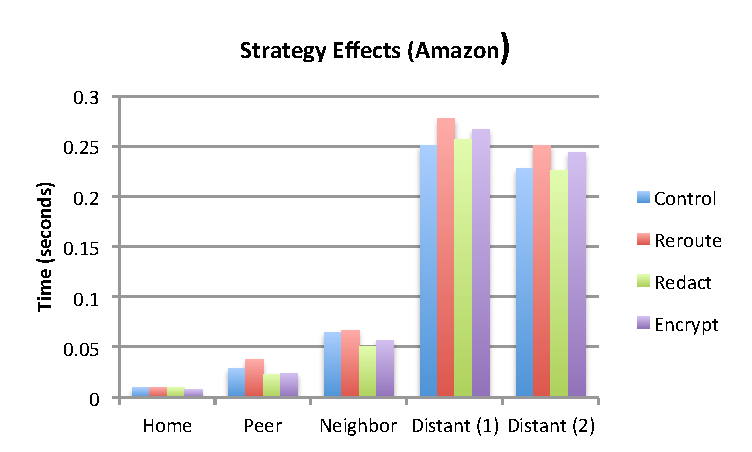
\includegraphics[width=6in]{strategy_effects_az}
\caption{Results from Amazon}
\label{fig:model:amazon-results}
\end{figure}

The goal of this experimental work was to characterize the issues around specific confidentiality strategies in these kinds of networks.  The specific strategies addressed were redaction, rerouting, and protection (via encryption), and we evaluated these strategies from the perspective of confidentiality, integrity, and availability. We measured confidentiality via the control used to protect information.  Removing information entirely provided the highest measure of protection but is akin to unplugging a computer to improve its cyber-security posture.   Routing information through a more secure channel is the next approach, followed by sensitive information protection via strong encryption.  We use 256-bit AES-CBC encryption scheme in our current work.  We measured availability by the delivery of information and the time required to ensure information delivery, measured by end-to-end network performance.  Integrity is a function of the alterations to the information required for secure delivery in the tested scenario.  Unaltered information has the highest integrity, followed by information that is still complete but protected via encryption, information that has been divided and rerouted, and finally information that has had content redacted.  Though we can specify combinations of strategies in a given network, as we specify strategies by network node, in our experiments we use a single strategy in each network to more clearly attribute strategy performance impacts. We used identical policies in each simulation to ensure the same amount of required usage management actions, limiting the effects on availability to the approach rather than differing policy.  We also ran a control simulation that did not incorporate any usage management to provide a performance baseline.  

Figure ~\ref{fig:model:amazon-results} shows our performance results from our Amazon testing node.  The access times for the content from the home, peer, and neighbor nodes were by far the smallest.  As the testing node was hosted in the same datacenter as these three nodes, that was to be expected.  The access times for both distant nodes was, however, surprisingly high.  With that in mind, the overall trend for response times is sensible however, with access time increasing as the requesting node is farther away from the content in the information network.  Queries from distant nodes need to traverse five information routers, while home, peer, and neighbor nodes only traverse one, two and three, respectively.  Also surprising was the finding that rerouting was generally more expensive from an availability perspective than encryption-based approaches.  This is likely attributable to the costs associated with attaching to the external SMTP server, hosted at Google, used as the out-of-band communications channel.  Also evident is remarkable performance variability.  Control data was collected at different times than experimental data, and infrastructural demands seem to have driven the control data availability to be less than that of other, managed approaches.  Overall, this evidence of variable performance due to external provider demands leads to the conclusion that overall, the availability costs of the various approaches are in fact negligible.

\begin{figure}[!t]
\centering
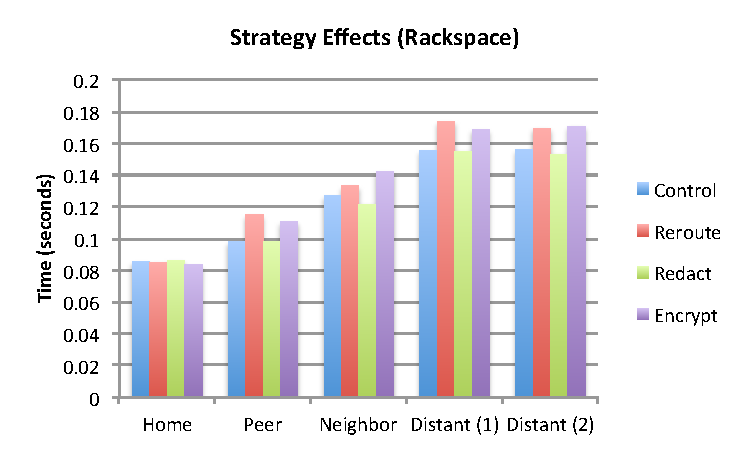
\includegraphics[width=6in]{strategy_effects_rs}
\caption{Results from Rackspace}
\label{fig:model:rackspace-results}
\end{figure}

Figure ~\ref{fig:model:rackspace-results} shows similar results to Figure ~\ref{fig:model:amazon-results}.  Here, the query times are much higher for the home and peer nodes, but actually lower for the distant nodes.  In this case, the content is still hosted in Amazon's infrastructure, but the testing node is at Rackspace.  As a result, the longer response time for content from the home node is to be expected.  Queries to distant nodes are actually shorter than the previous calls into distant nodes from Amazon.  This stems from the fact that the distant nodes are both hosted at Rackspace.  This locality shortens the round trip distance for a request.  Previously, from Amazon, a content request would need to travel from Amazon's east coast data centers to the Rackspace data center in Dallas, then back to the east coast for content, then back to Dallas, then back to the east cost.  In this test, the request only travels from Dallas to the east cost, and back.  Nevertheless, the overall performance profile is sensible, reflecting the expected shorter latency between home, peer, and neighbor nodes when compared to distant nodes.  Similar to amazon, we again have cases when the control latency is higher than experimental latency, indicating some amount of infrastructure performance variability.  In Figure ~\ref{fig:model:rackspace-results} however, we see that overall encryption and rerouting impact performance more than rerouting, as we would expect.  Rerouting again has high overall impact, likely as a result of contacting Google's remote SMTP services.

Figure ~\ref{fig:model:comcast-results} Shows performance results measured from Comcast.  Interestingly, they show significant variability when accessing nodes hosted at Amazon, and more predictable performance when accessing nodes in Rackspace's infrastructure.  The overall variability does not follow the expected pattern of shorter response times when accessing content from nodes close to that content, except in a few cases.  This illustrates the kind of performance variability one can expect from an external service provider.

Integrity impacts are the result of approach rather than platform.  Redacting content destroys information integrity, as information is removed and not delivered to requesters.  Encryption maintains integrity the best of the three alternatives as information, even though encrypted, is still delivered, and delivered in the context of the query response at that.  Rerouting is better than redaction, in that sensitive information is still delivered, but worse than encryption, as it is not delivered within the response context and is sent out-of-band. Simulations removed sensitive information from the information network and dispatched it to a user's email address via SMTP over TLS when the selected strategy was rerouting.  This impacts information availability, as email delivery times can be highly variable.  In our experiments, delivery could take anything from a few seconds to a few minutes.

\begin{figure}[!t]
\centering
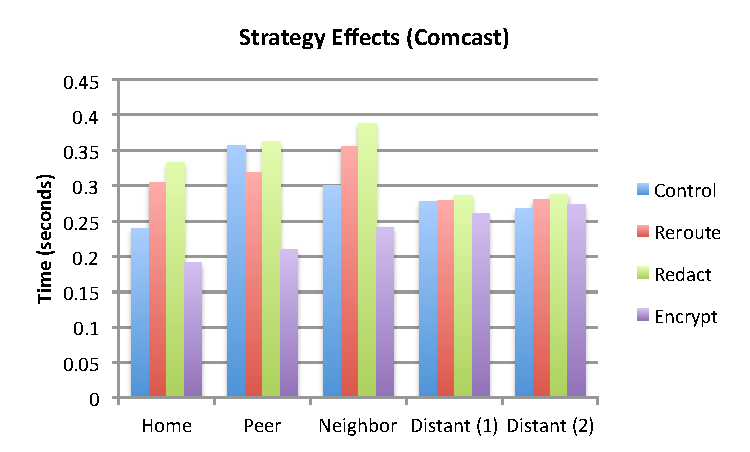
\includegraphics[width=6in]{strategy_effects_local}
\caption{Results from Comcast}
\label{fig:model:comcast-results}
\end{figure}

Confidentiality is likewise impacted primarily by approach and not by infrastructure.  Redacting sensitive content provides the best confidentiality protection, as sensitive content is simply not exposed.  Encryption is likely the worst solution from a confidentiality perspective as content encryption is a delaying tactic against a determined, well-resourced adversary.  Rerouting may be better or worse than encryption as an approach, depending on the confidentiality of the out-of-band channel.  If the security of that channel can be guaranteed, then it is likely a better approach.  If, on the other hand, the security of that channel is more variable or difficult to ascertain, encryption may be a more reliable approach.

Overall, our results show that, from a performance perspective, the encryption approach fares the worst, but only slightly, and certainly not in all cases.  Both our results from Amazon and Rackspace, in Figures ~\ref{fig:model:amazon-results} and ~\ref{fig:model:rackspace-results}, show encryption as generally taking the largest performance hit, just following rerouting.
Furthermore, network effects have a much larger impact on performance than information protection approaches.  The query to the home node is an excellent predictor of overall network stability, as content delivered directly from a home node is not subjected to the selected information protection strategy.  Note that when queried from Amazon or Rackspace, the home node timing results are very close to uniform.  Queries from Comcast, however, are much more varied, indicating more highly variable quality of service within the Comcast network.  This is also supported by the gross distribution of response times.  Within both the Amazon and Rackspace networks, the farther a queried node is from the content requested, the worse the performance, as expected.  Comcast's network has a much more uniform information network response time overall as the processing time of the information network simulation is overshadowed by the highly varied performance of Comcast's physical network.  Availability is surprisingly uniform across all confidentiality strategies, showing little impact on end-to-end processing times.  Encryption strategies show the most degradation, though that performance degradation is less than general network performance variation.

\begin{table*}[tp] %
\centering %
\begin{tabular}{lccc}
\toprule %
{\it Property}			& {\it Redaction}	& {\it Rerouting} 	& {\it Encryption} 	\\\toprule
{\it Infrastructure} 	& 3				  	& 1					& 1				 	\\\midrule
{\it Operating Systems}	& 1					& 2					& 3 				\\\midrule
{\it Technologies}		& 1					& 1					& 1					\\\bottomrule
\end{tabular}
\caption{Approach Evaluation Summary}
\label{table:model:evaluation}
\end{table*}

Table ~\ref{table:model:evaluation} shows the overall results of our experiments and analysis with respect to various possible approaches to securing information transiting content networks, on a scale of one to three, with three the highest and one the lowest scores.  Not surprisingly, there is no clear best approach.  Rather, decisions with respect to which approach to choose for given content is highly dependent on the sensitivity of the content as well as integrity and availability requirements.